\section{Contexto histórico e motivação}

%http://heroicrelics.org/info/v-2/v-2-cut-away.html
%https://v2rockethistory.com/?s=jet+vane

A tecnologia de empuxo vetorial (ou TVC, do inglês \textit{thrust vector control}) é chave para o setor aeroespacial, pois permite aproveitar o empuxo gerado pelo motor-foguete para aplicar um comando de atitude ao veículo. É uma tecnologia desenvolvida desde os primórdios da tecnologia de foguetes, com o míssil V2 sendo um marco notável no histórico do empuxo vetorial e dos foguetes. Este sistema, exibido na figura~\ref{fig:tvc_systems_jet_vanes}, utilizava lâminas de grafite (\textit{jet vanes}) inseridas na exaustão do motor principal para direcionar o escoamento de gases e produzir uma força lateral capaz de direcionar o míssil.

\begin{figure}
    \centering
    \begin{subfigure}{.49\textwidth}
        \centering
        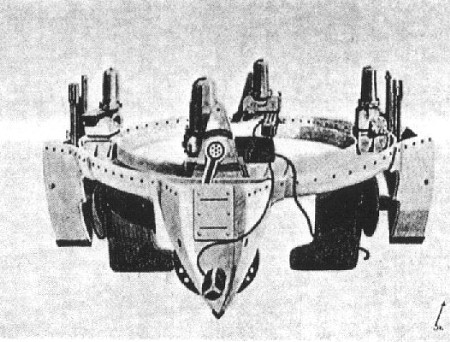
\includegraphics[width=.9\textwidth]{img/v2jetvanes.jpg}
        \caption{Sistema de \textit{jet vanes} do míssil V2~\cite{V2jetvanes}.}\label{fig:tvc_systems_jet_vanes}
    \end{subfigure}
    \hfill
    \begin{subfigure}{.49\textwidth}
        \centering
        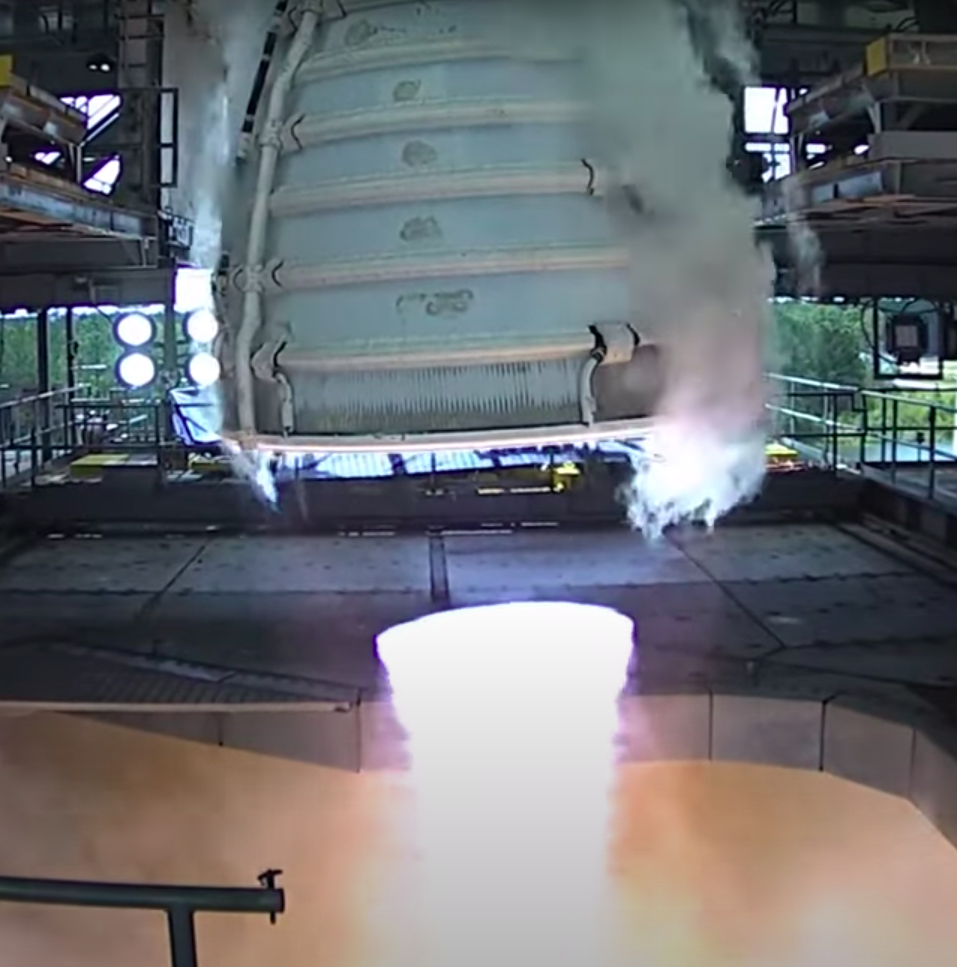
\includegraphics[width=.9\textwidth]{img/engine_gimbal.png}
        \caption{Sistema de \textit{gimbal} do motor RS-25 do foguete Artemis~\cite{RS25Gimbal}.}\label{fig:tvc_systems_gimbal}
    \end{subfigure}
    \caption{Exemplos de sistemas com empuxo vetorial.}
\end{figure}

Outros sistemas de empuxo vetorial foram desenvolvidos após a Segunda Guerra Mundial, tanto para aplicações militares como para lançadores de satélites, cada uma com seus \textit{trade-offs} de engenharia. Uma alternativa de alto desempenho e alta complexidade mecânica muito comum atualmente é a articulação esférica, ou \textit{gimbal}, da tubeira do motor. Um sistema \textit{gimbal}, do motor RS-25 desenvolvido para o ônibus espacial e reaproveitado para o programa Artemis, é exibido em ação na figura~\ref{fig:tvc_systems_gimbal}.

Os sistemas de empuxo vetorial são fundamentais para a estabilidade e para o seguimento de trajetória dos foguetes. Defeitos de manufatura podem introduzir desalinhamentos angulares e lineares de empuxo, que devem ser compensados pelo sistema de controle de empuxo vetorial. Também são fundamentais para o controle dos veículos em baixas velocidades, regime no qual aletas fornecem pouca ou nenhuma autoridade sobre o veículo, permitindo que se elimine a necessidade de trilhos de lançamento. Naturalmente, também funcionam no vácuo espacial. Este trabalho busca, portanto, iniciar uma linha de pesquisa brasileira sobre o assunto.

\section{Objetivos}

Este trabalho buscou desenvolver motor foguete a gás frio de pequena escala (2--5N), um sistema de empuxo vetorial baseado em \textit{jet vane} para direcionamento do empuxo em um plano, e a caracterização empírica das forças geradas pelo sistema, bem como as dificuldades identificadas para o desenvolvimento futuro do tema.